\section{Méthodes Agnostiques}

Séparer les explications du modèle d'apprentissage automatique (= model-agnostic interpretation models) présente certains avantages :

\begin{itemize}
    \item \textbf{Flexibilité du modèle :} La méthode d'interprétation peut fonctionner avec n'importe quel modèle d'apprentissage automatique, tels que les forêts aléatoires et les réseaux neuronaux profonds.
    
    \item \textbf{Flexibilité d'explication :} Vous n'êtes pas limité à une certaine forme d'explication. Dans certains cas, il peut être utile d'avoir une formule linéaire, dans d'autres cas, un graphique avec des importances de variables.
    
    \item \textbf{Flexibilité de représentation :} Le système d'explication devrait être capable d'utiliser différentes représentations des variables pour avoir une explication plus complète du modèle. 
\end{itemize}

\subsection{Graphique de Dépendance Partielle (PDP ou Partial Dependence Plot)}
Le graphique de dépendance partielle (abrégé PDP) montre l'effet marginal qu'une ou deux variables ont sur le résultat prédit d'un modèle d'apprentissage automatique.
\[ \hat{f}_S(x_S) = E_{X_C}\left[\hat{f}(x_S,X_C)\right] = \int \hat{f}(x_S,X_C) d\mathbb{P}(X_C) \]

Où \( x_S \) sont les variables pour lesquelles la fonction de dépendance partielle doit être tracée et \( X_C \) sont les autres variables utilisées dans le modèle d'apprentissage automatique \( \hat{f} \), qui sont ici traitées comme des variables aléatoires. Habituellement, il y a seulement une ou deux variables dans l'ensemble S.
La fonction partielle \( \hat{f}_S \) est estimée en calculant les moyennes dans les données d'entraînement, également connue sous le nom de méthode de Monte Carlo :

\[ \hat{f}_S(x_S) = \frac{1}{n} \sum_{i=1}^n \hat{f}(x_S,x^{(i)}_{C}) \]

La fonction partielle nous indique, pour des valeurs données des variables S, quel est l'effet marginal moyen sur la prédiction. Une hypothèse du PDP est que les variables dans C ne sont pas corrélées avec les variables dans S.


\begin{center}
    \centering
    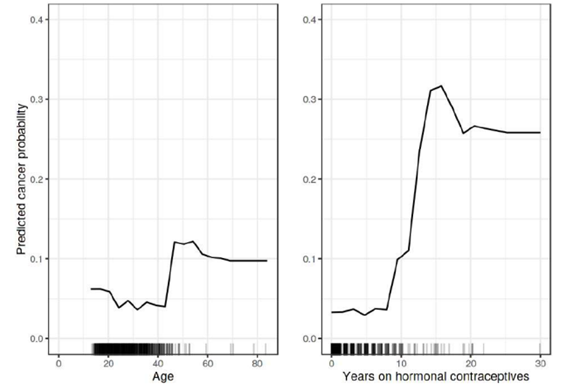
\includegraphics[width=0.7\linewidth]{Images/PDP.png}
    \\
    \emph{Figure 9: Partial Dependence Plot}
    \\
\end{center}
\\

\subsubsection{Avantages}
\begin{itemize}
    \item Le graphique de dépendance partielle est intuitif. Si la variable pour laquelle vous avez calculé le PDP n'est pas corrélée avec les autres variables, alors les PDPs représentent parfaitement comment la variable influence la prédiction en moyenne.
    \item Les graphiques de dépendance partielle sont faciles à mettre en œuvre.
    \item Le calcul pour les graphiques de dépendance partielle a une interprétation causale. Nous intervenons sur une variable et mesurons les changements dans les prédictions.
\end{itemize}

\subsubsection{Inconvénients}
\begin{itemize}
    \item Le nombre maximum réaliste de variables dans une fonction de dépendance partielle est de deux.
    \item Certains PDP ne montrent pas la distribution des variables.
    \item L'hypothèse d'indépendance est le plus gros problème avec les PDP.
    \item Les effets hétérogènes pourraient être cachés car les PDP montrent seulement les effets marginaux moyens.
\end{itemize}

\subsection{Individual Conditional Expectation (ICE)}
Les graphiques ICE affichent une ligne par instance qui montre comment la prédiction de l'instance change lorsqu'une variable change. Il équivaut à un PDP pour des instances de données individuelles.
Une définition plus formelle :
Dans les graphiques ICE, pour chaque instance dans \( \{(x_{S}^{(i)},x_{C}^{(i)})\}_{i=1}^N \), la courbe \( \hat{f}_S^{(i)} \) est tracée par rapport à \( x^{(i)}_{S} \), tandis que \( x^{(i)}_{C} \) reste fixe.


\begin{center}
    \centering
    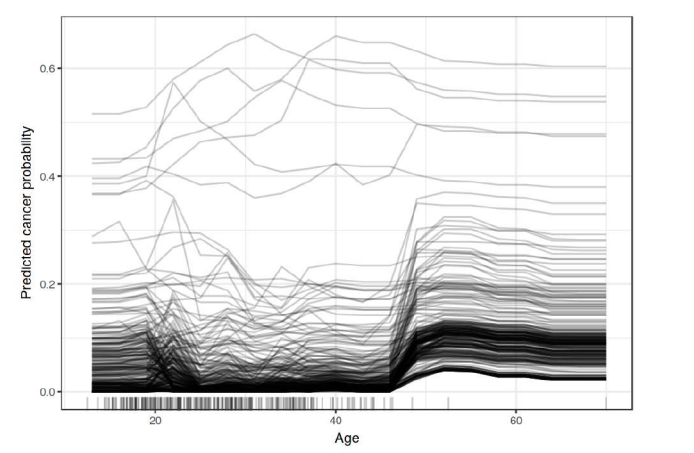
\includegraphics[width=0.7\linewidth]{Images/ice.png}
    \\
    \emph{Figure 10: ICE plot}
    \\
\end{center}
\\


\subsubsection{ICE centré}
Il y a un problème avec les graphiques ICE :
Parfois, il peut être difficile de dire si les courbes ICE diffèrent entre les individus parce qu'elles commencent à différentes prédictions. Une solution simple est de centrer les courbes :
\[ \hat{f}_{cent}^{(i)} = \hat{f}^{(i)} - \mathbf{1}\hat{f}(x^{a},x^{(i)}_{C}) \]
où \( \mathbf{1} \) est un vecteur de 1 ayant le nombre de dimensions approprié (généralement un ou deux), \( \hat{f} \) est le modèle ajusté et \( x^a \) est le point d'ancrage.

\begin{center}
    \centering
    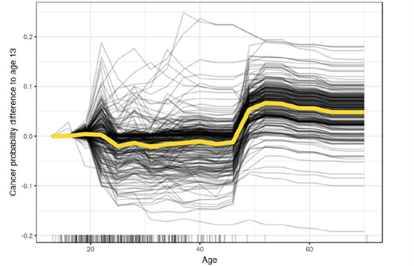
\includegraphics[width=0.7\linewidth]{Images/centered_ice.png}
    \\
    \emph{Figure 11: Centered ICE plot}
    \\
\end{center}
\\

\subsubsection{Graphique ICE dérivé}
Une autre façon de faciliter visuellement la détection de l'hétérogénéité est d'examiner les dérivées individuelles de la fonction de prédiction par rapport à une variable. Si aucune interaction n'existe entre la variable analysée \( x_S \) et les autres variables \( x_C \), alors la fonction de prédiction peut s'exprimer comme :
\[ \hat{f}(x) = \hat{f}(x_S,x_C) = g(x_S) + h(x_C), \quad\text{avec}\quad \frac{\delta\hat{f}(x)}{\delta{}x_S} = g'(x_S) \]
Sans interactions, les dérivées partielles individuelles devraient être les mêmes pour toutes les instances. Le problème est que le graphique ICE dérivé prend beaucoup de temps à calculer et est plutôt peu pratique.

\subsubsection{Avantages}
\begin{itemize}
    \item Les ICE plots sont encore plus intuitifs à comprendre que les graphiques de dépendance partielle. Une ligne représente les prédictions pour une instance si nous faisons varier la variable d'intérêt.
    \item Contrairement aux graphiques de dépendance partielle, les courbes ICE peuvent révéler des relations hétérogènes.
\end{itemize}

\subsubsection{Inconvénients}
\begin{itemize}
    \item Les courbes ICE ne peuvent afficher qu'une seule variable.
    \item Les courbes ICE souffrent du même problème que les PDPs : Si la variable d'intérêt est corrélée avec les autres variables, alors certains points des lignes pourraient être des points de données invalides selon la distribution conjointe des variables.
    \item Si de nombreuses courbes ICE sont tracées, le graphique peut devenir surchargé.
\end{itemize}


\subsection{Accumulated Local Effects (ALE) Plot}

Les effets locaux accumulés décrivent comment les variables influencent la prédiction d'un modèle d'apprentissage automatique en moyenne. Les graphiques ALE sont une alternative plus rapide et sans biais aux graphiques de dépendance partielle (PDPs).

\subsubsection{Motivation et Intuition}

Si les variables d'un modèle d'apprentissage automatique sont corrélées, le graphique de dépendance partielle ne peut pas être considéré comme fiable. Le calcul d'un graphique de dépendance partielle pour une variable fortement corrélée avec d'autres implique de moyenniser les prédictions de cas de données artificielles qui sont peu probables dans la réalité. 
\\
Pour résoudre ce problème, nous pouvons utiliser les M-Plots (ou Marginal-Plot, un nom qui prête à confusion, car ils sont basés sur la distribution conditionnelle, et non marginale). Ils calculent la moyenne des prédictions sur la distribution conditionnelle de la variable. Cependant, cela ne serait pas suffisant, supposons que nous prédisions la valeur d'une maison et supposons que la superficie habitable n'a aucun effet sur la valeur prédite d'une maison, seul le nombre de pièces en a. Le M-Plot montrerait toujours que la taille de la zone de vie augmente la valeur prédite, car le nombre de pièces (variable ayant un effet sur la valeur de la maison) augmente avec la superficie habitable. Les graphiques ALE résolvent ce problème en calculant (également sur la base de la distribution conditionnelle des variables) les différences de prédictions plutôt que les moyennes.

Pour résumer comment chaque type de graphique (PDP, M, ALE) calcule l'effet d'une variable à une certaine valeur de grille v : 

\begin{itemize}
    \item \textbf{Graphiques de dépendance partielle} : "Laissez-moi vous montrer ce que le modèle prédit en moyenne lorsque chaque cas de données a la valeur v pour cette variable. J'ignore si la valeur v a du sens pour tous les cas de données."
    \item \textbf{M-Plots} : "Laissez-moi vous montrer ce que le modèle prédit en moyenne pour les cas de données qui ont des valeurs proches de v pour cette variable. L'effet pourrait être dû à cette variable, mais aussi à des variables corrélées."
    \item \textbf{Graphiques ALE} : "Laissez-moi vous montrer comment les prédictions du modèle changent dans une petite ``fenêtre'' de la variable autour de v pour les cas de données dans cette fenêtre."
\end{itemize}



\subsubsection{Théorie}

Les graphiques de dépendance partielle font la moyenne des prédictions sur la distribution marginale.

\begin{align*}
\hat{f}_{S,PDP}(x)&=E_{X_C}\left[\hat{f}(x_S,X_C)\right] \\
& = \int_{X_C}\hat{f}(x_S,X_C)d\mathbb{P}(X_C)
\end{align*}

Les M-plots font la moyenne des prédictions sur la distribution conditionnelle.

\begin{align*}\hat{f}_{S,M}(x_S)&=E_{X_C|X_S}\left[\hat{f}(X_S,X_C)|X_S=x_s\right]\\&=\int_{X_C}\hat{f}(x_S, X_C)d\mathbb{P}(X_C|X_S = x_S)\end{align*}

Les graphiques ALE font la moyenne des changements dans les prédictions et les accumulent sur un interval (plus de détails sur le calcul plus tard).

\begin{align*}
\hat{f}_{S,ALE}(x_S)=&\int_{z_{0,S}}^{x_S}E_{X_C|X_S = x_S}\left[\hat{f}^S(X_s,X_c)|X_S=z_S\right]dz_S-\text{constant}\\
 = & \int_{z_{0,S}}^{x_S}(\int_{x_C}\hat{f}^S(z_s,X_c)d\mathbb{P}(X_C|X_S = z_S)d{})dz_S-\text{constant}
\end{align*}

La formule révèle trois différences par rapport aux M-plots. 
Premièrement, nous moyennons les changements de prédictions, et non les prédictions elles-mêmes.
Le changement est défini comme la dérivée partielle (mais remplacée plus tard, pour le calcul réel, par les différences dans les prédictions sur un intervalle).
$$\hat{f}^S(x_s,x_c)=\frac{\partial\hat{f}(x_S,x_C)}{\partial{}x_S}$$
La deuxième différence est l'intégrale supplémentaire sur z. Nous accumulons les gradients locaux sur la plage des variables dans l'ensemble S, ce qui nous donne l'effet de la variable sur la prédiction.
La troisième différence des graphiques ALE par rapport aux M-plots est que nous soustrayons une constante des résultats. Cette étape centre le graphique ALE de sorte que l'effet moyen sur les données est nul. Un problème demeure : Tous les modèles n'ont pas un gradient, par exemple, les forêts aléatoires n'en ont pas. Mais comme vous le verrez, le calcul réel fonctionne sans gradients et utilise des intervalles.

\paragraph{Estimation}
\\

Je vais d'abord décrire comment les graphiques ALE sont estimés pour une seule variable numérique, puis pour deux variables numériques et pour une seule variable catégorielle. Pour estimer les effets locaux, nous divisons la variable en de nombreux intervalles et calculons les différences dans les prédictions. Cette procédure approxime les gradients et fonctionne également pour les modèles sans gradients.
Tout d'abord, nous estimons l'effet non centré : 
$$\hat{\tilde{f}}_{j,ALE}(x)=\sum_{k=1}^{k_j(x)}\frac{1}{n_j(k)}\sum_{i:x_{j}^{(i)}\in{}N_j(k)}\left[\hat{f}(z_{k,j},x^{(i)}_{-j})-\hat{f}(z_{k-1,j},x^{(i)}_{-j})\right]$$
Le nom \textbf{Effets Locaux Accumulés} reflète bien tous les composants individuels de cette formule.
Au cœur de la méthode ALE, on calcule les différences dans les prédictions, où l'on remplace la variable d'intérêt par des valeurs de grille z.
La différence de prédiction est l'\textbf{Effet} que la variable a pour une instance individuelle dans un certain intervalle.
La somme à droite ajoute les effets de toutes les instances à l'intérieur d'un intervalle qui apparaît dans la formule comme voisinage \(N_j(k)\).
Nous divisons cette somme par le nombre d'instances dans cet intervalle pour obtenir la différence moyenne des prédictions pour cet intervalle.
Cette moyenne dans l'intervalle est couverte par le terme \textbf{Local} dans le nom ALE.
Le symbole de somme à gauche signifie que nous accumulons les effets moyens sur tous les intervalles.
L'effet (non centré) d'une valeur de variable qui se trouve, par exemple, dans le troisième intervalle est la somme des effets du premier, du deuxième et du troisième intervalles.
Le mot \textbf{Accumulé} dans ALE reflète cela.
Cet effet est centré de sorte que l'effet moyen est nul.
$$\hat{f}_{j,ALE}(x)=\hat{\tilde{f}}_{j,ALE}(x)-\frac{1}{n}\sum_{i=1}^{n}\hat{\tilde{f}}_{j,ALE}(x^{(i)}_{j})$$
La valeur de l'ALE peut être interprétée comme l'effet principal de la variable à une certaine valeur par rapport à la prédiction moyenne des données.

\subsubsection{Avantages}

Les graphiques ALE sont sans biais, ce qui signifie qu'ils fonctionnent toujours lorsque les variables sont corrélées.
Les graphiques ALE sont plus rapides à calculer que les PDPs et évoluent avec O(n).
L'interprétation des graphiques ALE est claire : Conditionnellement à une valeur donnée, l'effet relatif de la modification de la variable sur la prédiction peut être lu à partir du graphique ALE. Les graphiques ALE sont centrés à zéro. Cela rend leur interprétation agréable, car la valeur à chaque point de la courbe ALE est la différence par rapport à la prédiction moyenne.
Dans l'ensemble, dans la plupart des situations, je préférerais les graphiques ALE aux PDPs, car les variables sont généralement corrélées à un certain degré.

\subsubsection{Inconvénients}

Les graphiques ALE peuvent devenir un peu instables (beaucoup de petits hauts et bas) avec un grand nombre d'intervalles.
Il n'y a pas de solution parfaite pour fixer le nombre d'intervalles.
Les graphiques ALE ne sont pas accompagnés de courbes ICE (plus difficile de vérifier l'hétérogénéité).
L'implémentation des graphiques ALE est beaucoup plus complexe et moins intuitive que celle des graphiques de dépendance partielle.
Même si les graphiques ALE ne sont pas biaisés en cas de variables corrélées, l'interprétation reste difficile lorsque les variables sont fortement corrélées.

\subsection{Feature Interaction}

Lorsque des variables interagissent entre elles dans un modèle de prédiction, la prédiction ne peut pas être exprimée comme la somme des effets des variables. 

\subsubsection{Théorie : Statistique H de Friedman}
Si deux variables n'interagissent pas, nous pouvons décomposer la fonction de dépendance partielle comme suit (en supposant que les fonctions de dépendance partielle sont centrées à zéro):

\[
PD_{jk}(x_j,x_k) = PD_j(x_j) + PD_k(x_k)
\]

où \(PD_{jk}(x_j,x_k)\) est la fonction de dépendance partielle (pour deux variables) pour j et k et \(PD_j(x_j)\) et \(PD_k(x_k)\) sont les fonctions de dépendance partielle des variables uniques.

De même, si une variable n'a aucune interaction avec aucune des autres variables, nous pouvons exprimer la fonction de prédiction \(\hat{f}(x)\) comme une somme de fonctions de dépendance partielle, où le premier terme ne dépend que de j et le second de toutes les autres variables sauf j :

\[
\hat{f}(x) = PD_j(x_j) + PD_{-j}(x_{-j})
\]

où \(PD_{-j}(x_{-j})\) est la fonction de dépendance partielle qui dépend de toutes les variables sauf de la j-ième variable.

Cette décomposition exprime la dépendance partielle (ou prédiction complète) sans interactions (entre les variables j et k, ou respectivement j et toutes les autres variables).

Nous calculons la variance de la sortie de la dépendance partielle (pour mesurer l'interaction entre deux variables) ou de la fonction entière (pour mesurer l'interaction entre une variable et toutes les autres variables).

Le montant de la variance expliquée par l'interaction (différence entre la PD observée et la PD sans interaction) est utilisé comme statistique de force d'interaction.

La statistique est 0 s'il n'y a aucune interaction du tout et 1 si toute la variance de \(PD_{jk}\) ou \(\hat{f}\) est expliquée par la somme des fonctions de dépendance partielle.

Mathématiquement, la statistique H proposée par Friedman et Popescu pour l'interaction entre la variable j et k est :

\[
H^2_{jk} = \frac{\sum_{i=1}^n\left[PD_{jk}(x_{j}^{(i)},x_k^{(i)}) - PD_j(x_j^{(i)}) - PD_k(x_{k}^{(i)})\right]^2}{\sum_{i=1}^n{PD^2_{jk}(x_j^{(i)},x_k^{(i)})}}
\]

La même chose s'applique pour mesurer si une variable j interagit avec n'importe quelle autre variable :

\[
H^2_{j} = \frac{\sum_{i=1}^n\left[\hat{f}(x^{(i)}) - PD_j(x_j^{(i)}) - PD_{-j}(x_{-j}^{(i)})\right]^2}{\sum_{i=1}^n\hat{f}^2(x^{(i)})}
\]

La statistique H est coûteuse à évaluer, car elle itère sur tous les points de données et à chaque point la dépendance partielle doit être évaluée ce qui est fait avec tous les n points de données.

Dans le pire des cas, nous avons besoin de \(2n^2\) appels à la fonction de prédiction du modèle d'apprentissage automatique pour calculer la statistique H à deux voies (j contre k) et \(3n^2\) pour la statistique H totale (j contre tous).

Pour accélérer le calcul, nous pouvons échantillonner parmi les n points de données. Cela a l'inconvénient d'augmenter la variance des estimations de dépendance partielle, ce qui rend la statistique H instable. Après avoir examiné les interactions des valeurs de chaque variable avec toutes les autres variables, nous pouvons sélectionner l'une des variables et approfondir toutes les interactions à deux variables entre la variable sélectionnée et les autres variables.

\begin{center}
    \centering
    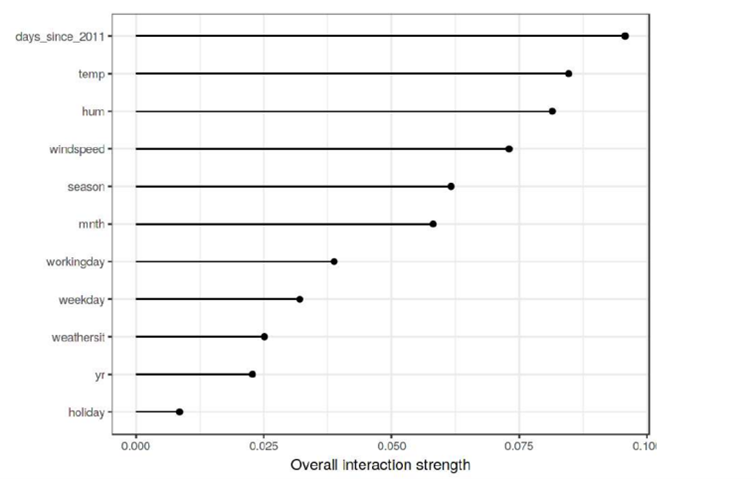
\includegraphics[width=0.7\linewidth]{Images/h_stat.png}
    \\
    \emph{Figure 12: H-Stat example}
    \\
\end{center}
\\


\subsubsection{Avantages}
La statistique d'interaction H a une \textbf{théorie sous-jacente} à travers la décomposition de la dépendance partielle.
La statistique H a une \textbf{interprétation significative} :
L'interaction est définie comme la part de variance qui est expliquée par l'interaction.
Puisque la statistique est \textbf{sans dimension}, elle est comparable entre les variables et même entre les modèles.

\subsubsection{Inconvénients}
Elle est coûteuse en calcul.
Ces estimations ont également une certaine variance si nous n'utilisons pas tous les points de données. Cela signifie que lorsque nous échantillonnons des points, les estimations varient également d'une exécution à l'autre et les résultats peuvent être instables.

Il n'est pas clair si une interaction est significativement supérieure à 0.
Concernant le problème test, il est difficile de dire quand la statistique H est suffisamment grande pour que nous considérions une interaction comme "forte".
La statistique H nous indique la force des interactions, mais elle ne nous dit pas à quoi ressemblent les interactions. Une approche significative consiste à mesurer les forces d'interaction puis à créer des tracés de dépendance partielle en 2D pour les interactions qui nous intéressent.

\subsubsection{Alternatives}
Les Variable Interaction Networks (VIN) de Hooker (2004) sont une approche qui décompose la fonction de prédiction en effets principaux et interactions entre variables. Les interactions entre les variables sont ensuite visualisées comme un réseau. Malheureusement, aucune implémentation de cette approche n'est encore disponible.



\subsection{Feature Importance}

\subsubsection{Théorie:}
Nous mesurons l'importance d'une variable en calculant l'augmentation de l'erreur de prédiction du modèle après avoir permuté la variable. Une variable est "importante" si mélanger ses valeurs augmente l'erreur du modèle, car dans ce cas, le modèle s'est appuyé sur la variable pour la prédiction.

\paragraph{L'algorithme d'importance de permutation des variables basé sur Fisher, Rudin, et Dominici (2018):}

\begin{enumerate}
    \item Estimer l'erreur du modèle d'origine $e_{orig} = L(y, \hat{f}(X))$  (par exemple, l'erreur quadratique moyenne).
    \item Pour chaque variable $j \in \{1,...,p\}$:
    \begin{itemize}
        \item Générer la matrice de variables $X_{perm}$ en permutant la variable j dans les données X. Cela rompt l'association entre la variable j et le véritable résultat y.
        \item Estimer l'erreur $e_{perm} = L(Y,\hat{f}(X_{perm}))$ basée sur les prédictions des données permutées.
        \item Calculer l'importance de permutation des variables comme quotient $FI_j= e_{perm}/e_{orig}$ ou différence $FI_j = e_{perm}- e_{orig}$.
    \end{itemize}
    \item Trier les variables par FI (feature impoortance) décroissant.
\end{enumerate}

\textbf{Dois-je calculer la FI sur les données d'entraînement ou de test?}

Le calcul de la FI basé sur les données d'entraînement nous fait croire à tort que les variables sont importantes pour les prédictions, alors qu'en réalité le modèle overfit et les variables n'étaient pas importantes du tout. La FI basée sur les données d'entraînement nous indique quelles variables sont importantes pour le modèle dans le sens où il dépend d'elles pour faire des prédictions.
En fin de compte, vous devez décider si vous voulez savoir dans quelle mesure le modèle s'appuie sur chaque variable pour faire des prédictions (-> données d'entraînement) ou dans quelle mesure la variable contribue à la performance du modèle sur des données non vues (-> données de test).

\subsubsection{Avantages:}
\begin{itemize}
    \item \textbf{Belle interprétation}: La FI est l'augmentation de l'erreur du modèle lorsque l'information de la variable est détruite.
    \item L'importance des variables offre un \textbf{aperçu global hautement compressé} du comportement du modèle.
    \item Un aspect positif de l'utilisation du ratio d'erreur plutôt que de la différence d'erreur est que les mesures d'importance des variables sont \textbf{comparables à travers différents problèmes}.
    \item La mesure d'importance prend automatiquement en compte \textbf{toutes les interactions} avec d'autres variables. En permutant la variable, vous détruisez également les effets d'interaction avec d'autres variables.
\end{itemize}

\subsubsection{Inconvénients:}
\begin{itemize}
    \item L'importance de permutation des variables est liée à l'erreur du modèle. Ce n'est pas intrinsèquement mauvais, mais dans certains cas, ce n'est pas ce dont vous avez besoin.
    \item Vous avez besoin d'accéder au véritable résultat. Si quelqu'un ne vous fournit que le modèle et des données non étiquetées - mais pas le véritable résultat - vous ne pouvez pas calculer l'importance de permutation des variables.
    \item L'importance de permutation des variables dépend du mélange de la variable, ce qui ajoute de l'aléatoire à la mesure. Lorsque la permutation est répétée, les résultats peuvent varier considérablement.
    \item Si les variables sont corrélées, l'importance de permutation des variables peut être biaisée par des instances de données irréalistes.
    \item Autre subtilité: Ajouter une variable corrélée peut diminuer la FI en splittant l'importancee associée aux deux variables.
\end{itemize}

\subsection{Global Surrogate Model}

Un modèle substitut global (Global Surrogate Model) est un modèle interprétable qui est entraîné pour approximer les prédictions d'un modèle boîte noire.

\subsubsection{Théorie:}

L'objectif des modèles substituts (interprétables) est d'approximer le plus précisément possible les prédictions du modèle sous-jacent tout en étant interprétables. Pour obtenir un modèle substitut, suivez les étapes suivantes:

\begin{enumerate}
    \item Sélectionnez un ensemble de données $X$. Cela peut être le même ensemble de données qui a été utilisé pour l'entraînement du modèle boîte noire ou un nouvel ensemble de données de la même distribution.
    \item Pour l'ensemble de données $X$ sélectionné, obtenez les prédictions du modèle boîte noire.
    \item Sélectionnez un type de modèle interprétable (modèle linéaire, arbre de décision, ...).
    \item Entraînez le modèle interprétable sur l'ensemble de données $X$ et ses prédictions.
    \item Félicitations! Vous avez maintenant un modèle substitut.
    \item Mesurez à quel point le modèle substitut réplique les prédictions du modèle boîte noire.
    \item Interprétez le modèle substitut.
\end{enumerate}

Une façon de mesurer la fidélité du substitut par rapport au modèle boîte noire est la mesure $R^2$:

\[
R^2 = 1 - \frac{\sum_{i=1}^n (\hat{y}_*^{(i)} - \hat{y}^{(i)})^2}{\sum_{i=1}^n (\hat{y}^{(i)} - \bar{\hat{y}})^2}
\]

où $\hat{y}_*^{(i)}$ est la prédiction pour la i-ème instance du modèle substitut, $\hat{y}^{(i)}$ est la prédiction du modèle boîte noire et $\bar{\hat{y}}$ est la moyenne des prédictions du modèle boîte noire.

\subsubsection{Avantages:}
\begin{itemize}
    \item La méthode du modèle substitut est flexible: tout modèle du chapitre sur les modèles interprétables peut être utilisé.
    \item La méthode est intuitive et directe.
    \item Avec la mesure $R^2$, nous pouvons facilement mesurer la qualité de nos modèles substituts.
\end{itemize}

\subsubsection{Inconvénients:}
\begin{itemize}
    \item Il faut être conscient que l'on tire des conclusions sur le modèle et non sur les données, puisque le modèle substitut n'a jamais accès au véritable résultat.
    \item Le seuil optimal pour $R^2$ n'est pas clair.
    \item Il se pourrait que le modèle interprétable soit très précis pour un sous-ensemble de données mais diverge considérablement pour un autre.
\end{itemize}



\subsection{Modèle Substitut Local (LIME)}

\subsubsection{Introduction}

Les modèles substituts locaux sont des modèles interprétables utilisés pour expliquer les prédictions individuelles des modèles d'apprentissage automatique de boîte noire. Au lieu d'entraîner un modèle substitut global, LIME se concentre sur l'entraînement de modèles substituts locaux.

\subsubsection{Définition mathématique}

Mathématiquement, les modèles substituts locaux avec contrainte d'interprétabilité peuvent être exprimés comme suit :
\[ \text{explication}(x) = \arg\min_{g\in{}G}L(f,g,\pi_x)+\Omega(g) \]
L'explication du modèle pour l'instance \( x \) est le modèle \( g \) (par exemple, un modèle de régression linéaire) qui minimise la perte \( L \) (par exemple, l'erreur quadratique moyenne), mesurant la proximité de l'explication par rapport à la prédiction du modèle original \( f \) tout en maintenant la complexité du modèle \( \Omega(g) \) faible.
G est la famille des explications possibles, par exemple tous les modèles de régression linéaire possibles.
La mesure de proximité $\pi_x$ définit la taille du voisinage de l'instance x que nous considérons pour l'explication.
\subsubsection{Procédure}

La procédure pour entraîner des modèles substituts locaux est la suivante :
\begin{enumerate}
    \item Sélectionnez votre instance d'intérêt.
    \item Perturbez votre jeu de données et obtenez les prédictions pour ces nouveaux points.
    \item Pesez les nouveaux échantillons selon leur proximité avec l'instance d'intérêt.
    \item Entraînez un modèle interprétable pondéré sur l'ensemble de données.
    \item Expliquez la prédiction en interprétant le modèle local.
\end{enumerate}

À l'avance, vous devez sélectionner K, le nombre de variables que vous souhaitez avoir dans votre modèle interprétable. Plus K est faible, plus il est facile d'interpréter le modèle. Un K plus élevé produit potentiellement des modèles plus fidèles. Il existe plusieurs méthodes pour former des modèles avec exactement K variables. Un bon choix est Lasso. D'autres stratégies consistent à sélectionner les variables en avant ou en arrière.

\paragraph{Comment obtenir les variations des données ?} Cela dépend du type de données, qui peuvent être des textes, des images ou des tableaux. Pour les textes et les images, la solution consiste à activer ou désactiver les mots isolés ou les super-pixels. Dans le cas des données tabulaires, LIME crée de nouveaux échantillons en perturbant chaque variable individuellement, en puisant dans une distribution normale dont la moyenne et l'écart type sont tirés de la variable.

\subsubsection{Applications de LIME}

\paragraph{Pour les données tabulaires: }

La définition d'un voisinage significatif autour d'un point est difficile. LIME utilise actuellement un noyau de lissage exponentiel pour définir le voisinage.
Algorithme LIME pour les données tabulaires. 
A) Prédictions de la forêt aléatoire à partir des variables x1 et x2. Classes prédites : 1 (couleur foncée) ou 0 (couleur claire). 
B) Instance d'intérêt (point jaune) et données échantillonnées à partir d'une distribution normale (points noirs). 
C) Attribuer un poids plus élevé aux points proches de l'instance d'intérêt. 
D) Les couleurs et les signes de la grille indiquent les classifications du modèle appris localement à partir des échantillons pondérés. La ligne blanche marque la limite de décision (P(class=1) = 0,5).
\begin{center}
    \centering
    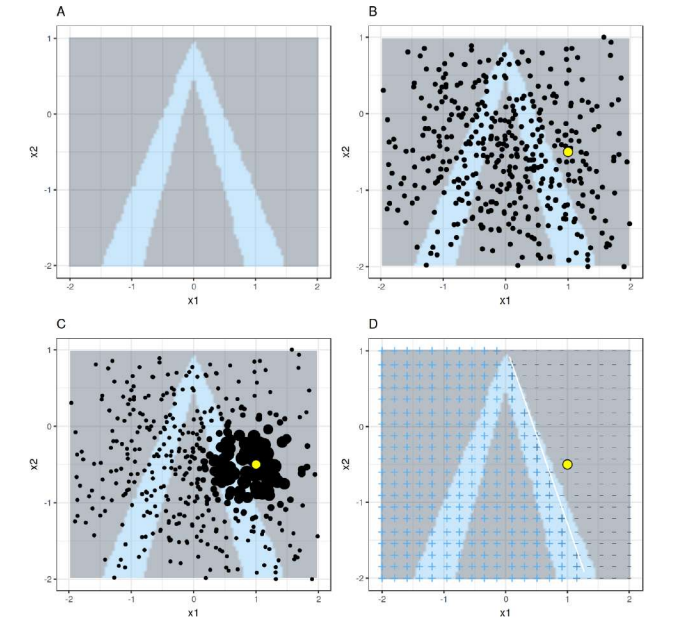
\includegraphics[width=0.7\linewidth]{Images/lime.png}
    \\
    \emph{Figure 13: Protocole d'un modèle LIME}
    \\
\end{center}
\\

Il est difficile de définir un voisinage significatif autour d'un point. LIME utilise actuellement un noyau de lissage exponentiel pour définir le voisinage. 

Si vous regardez l'implémentation Python de LIME, la largeur du noyau est de 0,75 fois la racine carrée du nombre de colonnes des données d'apprentissage.
\begin{center}
    \centering
    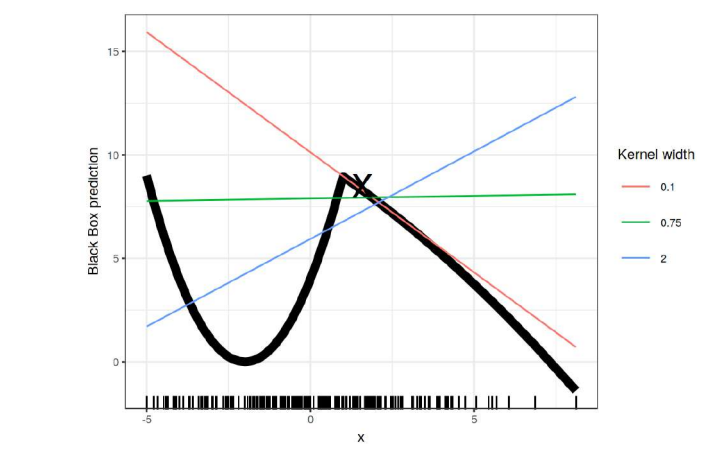
\includegraphics[width=0.7\linewidth]{Images/lime_width.png}
    \\
    \emph{Figure 14: Prédiction selon la largeur du noyau}
    \\
\end{center}
\\

\paragraph{Pour le texte: }

À partir du texte original, de nouveaux textes sont créés en supprimant aléatoirement des mots. Le jeu de données est représenté par des variables binaires pour chaque mot.

\paragraph{Pour les images: }

Les variations des images sont créées en segmentant l'image en "superpixels" et en les activant ou désactivant. Les superpixels sont des pixels interconnectés avec des couleurs similaires.

\subsubsection{Avantages}

Parmi les avantages de LIME, on trouve :
\begin{itemize}
    \item L'indépendance par rapport au modèle de machine learning sous-jacent.
    \item La création d'explications adaptées à l'homme.
    \item La mesure de fidélité offrant une idée fiable du modèle interprétable.
    \item La flexibilité pour travailler avec des données tabulaires, du texte et des images.
    \item L'implémentation facile en Python et R.
\end{itemize}

\subsubsection{Inconvénients}

Les inconvénients comprennent :
\begin{itemize}
    \item La difficulté de définir correctement le voisinage avec des données tabulaires.
    \item La nécessité de définir la complexité du modèle d'explication à l'avance.
\end{itemize}


\subsection{Valeurs de Shapley}

\subsubsection{Idée Générale}
La valeur de Shapley, introduite par Shapley en 1953, est une méthode permettant d'attribuer des paiements aux joueurs en fonction de leur contribution au paiement total. Le « jeu » est la tâche de prédiction pour une seule instance de l'ensemble de données. Le « gain » est la prédiction réelle pour cette instance moins la prédiction moyenne pour toutes les instances. Les « joueurs » sont les valeurs des variables de l'instance qui collaborent pour recevoir le gain ( = prédire une certaine valeur). La valeur de Shapley est la contribution marginale moyenne d'une valeur de variable parmi toutes les coalitions possibles. Le temps de calcul augmente de façon exponentielle avec le nombre de variables.

\subsubsection{La Valeur de Shapley}
La valeur de Shapley d'une valeur de variable est sa contribution au paiement, pondérée et sommée sur toutes les combinaisons possibles de valeurs de variables :
\[
\phi_j(val)=\sum_{{S\subseteq\{1,\ldots,p\} \backslash \{j\}}}\frac{{|S|!(p-|S|-1)!}}{{p!}}\left(val\left(S\cup\{j\}\right)-val(S)\right)
\]
où \( S \) est un sous-ensemble des variables utilisées dans le modèle, \( x \) est le vecteur des valeurs des variables de l'instance à expliquer et \( p \) le nombre de variables.
\( val_x(S) \) est la prédiction pour les valeurs de variables dans l'ensemble \( S \) qui sont marginalisées sur les variables qui ne sont pas incluses dans l'ensemble \( S \) :
\[
val_{x}(S)=\int\hat{f}(x_{1},\ldots,x_{p})d\mathbb{P}_{x\notin{}S}-E_X(\hat{f}(X))
\]

\subsubsection{Propriétés}
\textbf{Efficience} : Les contributions des variables doivent s'additionner à la différence de prédiction pour \( x \) et la moyenne.
\[
\sum\nolimits_{{j=1}}^p\phi_j=\hat{f}(x)-E_X(\hat{f}(X))
\]

\textbf{Symétrie} : Les contributions de deux valeurs de variables \( j \) et \( k \) doivent être les mêmes si elles contribuent également à toutes les coalitions possibles.
Si \( val(S \cup \{j\})=val(S\cup\{k\}) \) pour tous \( S\subseteq\{1,\ldots, p\} \backslash \{j,k\} \), alors \( \phi_j=\phi_{k} \).

\textbf{Joueur inactif} : Une variable \( j \) qui ne change pas la valeur prédite, quelles que soient les valeurs de variables auxquelles elle est ajoutée, devrait avoir une valeur de Shapley de 0.
Si \( val(S\cup\{j\})=val(S) \) pour tous \( S\subseteq\{1,\ldots,p\} \), alors \( \phi_j=0 \).

\textbf{Additivité} : Pour un jeu avec des paiements combinés \( val+val^{+} \), les valeurs de Shapley respectives sont les suivantes : \( \phi_j+\phi_j^{+} \). 
Supposons que vous ayez entraîné une forêt aléatoire, ce qui signifie que la prédiction est une moyenne de plusieurs arbres de décision. La propriété d'additivité garantit que pour une valeur de variable, vous pouvez calculer la valeur de Shapley pour chaque arbre individuellement, les moyennez, et obtenir la valeur de Shapley pour la valeur de variable pour la forêt aléatoire.

\subsubsection{Estimation de la Valeur de Shapley}
Strumbelj et al. (2014) proposent une approximation avec un échantillonnage Monte-Carlo:
\[
\hat{\phi}_{j}=\frac{1}{M}\sum_{m=1}^{M}\left(\hat{f}(x^{m}_{+j})-\hat{f}(x^{m}_{-j})\right)
\]
où \( \hat{f}(x^{m}_{+j}) \) est la prédiction pour \( x \), mais avec un certain nombre aléatoire de valeurs de variables remplacées par les valeurs de variables d'un point de données aléatoire \( z \), sauf pour la valeur respective de la variable \( j \).
Le vecteur \( x^{m}_{-j} \) est presque identique à \( x^{m}_{+j} \), mais la valeur \( x_j^{m} \) est également tirée de \( z \) échantillonné.
\\
\textbf{Estimation approximative de Shapley pour une seule valeur de variable}:
\begin{itemize}
  \item Output : Valeur de Shapley pour la valeur de la \( j \)-ième variable
  \item Requis : Nombre d'itérations \( M \), instance d'intérêt \( x \), indice de variable \( j \), matrice de données \( X \), et modèle d'apprentissage automatique \( f \)
  \begin{itemize}
    \item Pour tout \( m = 1,...,M \):
    \begin{itemize}
      \item Tirer une instance aléatoire \( z \) de la matrice de données \( X \)
      \item Choisir une permutation aléatoire \( o \) des valeurs de variables
      \item Ordonner l'instance \( x \): \( x_o = (x_{(1)},\ldots,x_{(j)},\ldots,x_{(p)}) \)
      \item Ordonner l'instance \( z \): \( z_o = (z_{(1)},\ldots,z_{(j)},\ldots,z_{(p)}) \)
      \item Construire deux nouvelles instances
      \begin{itemize}
        \item Avec \( j \): \( x_{+j} = (x_{(1)},\ldots,x_{(j-1)},x_{(j)},z_{(j+1)},\ldots,z_{(p)}) \)
        \item Sans \( j \): \( x_{-j} = (x_{(1)},\ldots,x_{(j-1)},z_{(j)},z_{(j+1)},\ldots,z_{(p)}) \)
      \end{itemize}
      \item Calculer la contribution marginale : \( \phi_j^{m}=\hat{f}(x_{+j})-\hat{f}(x_{-j}) \)
    \end{itemize}
    \item Calculer la valeur de Shapley comme la moyenne : \( \phi_j(x)=\frac{1}{M}\sum_{m=1}^{M}\phi_j^{m} \)
  \end{itemize}
\end{itemize}

\subsection{Avantages}
\begin{itemize}
  \item La différence entre la prédiction et la prédiction moyenne est équitablement répartie parmi les valeurs de variables de l'instance ie la propriété d'Efficience des valeurs de Shapley.
  \item La valeur de Shapley permet des explications contrastives.
  \item La valeur de Shapley est une des seules méthodes d'explication avec une théorie solide.
\end{itemize}

\subsection{Inconvénients}
\begin{itemize}
  \item La valeur de Shapley nécessite beaucoup de temps de calcul. Dans 99,9\% des problèmes du monde réel, seule la solution approximative est réalisable.
  \item Les explications créées avec la méthode de la valeur de Shapley utilisent toujours toutes les variables.
  \item La valeur de Shapley retourne une simple valeur par variable, mais pas un modèle de prédiction comme LIME.
  \item Un autre inconvénient est que vous devez avoir accès aux données si vous souhaitez calculer la valeur de Shapley pour une nouvelle instance de données.
  \item Comme beaucoup d'autres méthodes d'interprétation basées sur la permutation, la méthode de la valeur de Shapley souffre de l'inclusion de cas de données irréalistes lorsque les variables sont corrélées.
\end{itemize}
